\documentclass{article}
\usepackage[margin=1in]{geometry}
\usepackage{amsmath}
\usepackage{graphicx}
\usepackage{float}
\usepackage{listings}
\usepackage{xcolor}

\lstset{
    language=Matlab,
    basicstyle=\ttfamily\footnotesize,
    keywordstyle=\color{blue},
    breaklines=true
}

\begin{document}

\section*{Problem 1(b)}

The steady-state advection-diffusion problem is solved using a nonuniform mesh with $E=20$ elements. The element lengths follow a geometric progression $L_e = s L_{e-1}$ with a scale factor of $s=0.7$. The length of the first element is determined by the geometric series sum:
\begin{equation}
    L_1 = L \frac{1 - s}{1 - s^E}
\end{equation}

\subsection*{Results}
By geometrically clustering the elements near the right boundary ($x=1$), the local element P\'eclet number in the steep boundary layer region is significantly reduced. This mitigates the spatial oscillations observed in the uniform mesh approach. The computed maximum pointwise relative error is \textbf{0.0120} ($1.1972 \times 10^{-2}$).

\begin{figure}[H]
    \centering
    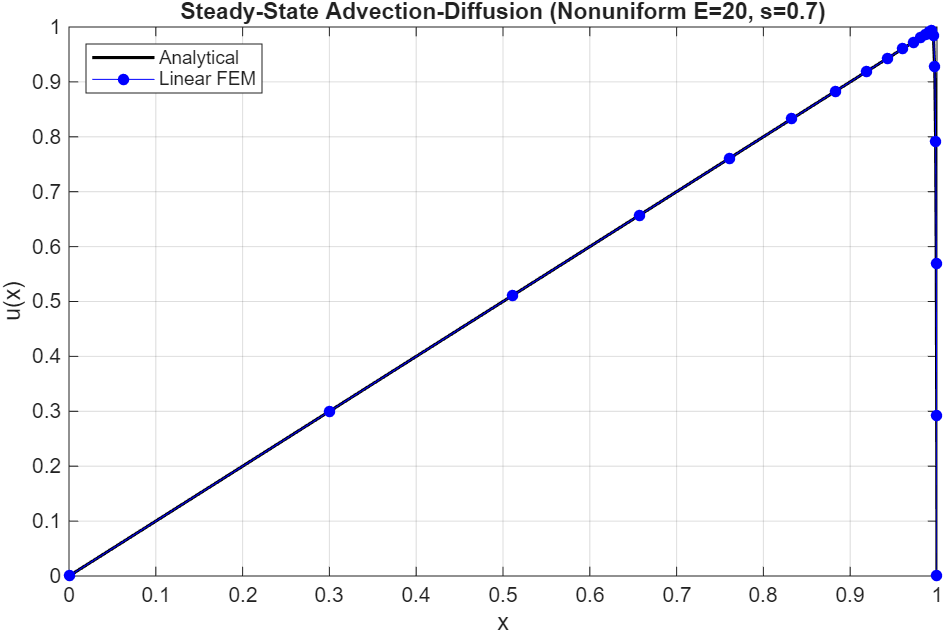
\includegraphics[width=0.7\textwidth]{1_b.png}
    \caption{Steady-State Advection-Diffusion using a nonuniform mesh ($E=20, s=0.7$).}
    \label{fig:1b}
\end{figure}

\subsection*{MATLAB Implementation}
\begin{lstlisting}
L = 1.0; c = 1.0; nu = 1e-3; f = 1.0;
E = 20; N = E + 1; s = 0.7;

L1 = L * (1 - s) / (1 - s^E);
Le = L1 * s.^(0:E-1);
x = [0, cumsum(Le)]';

K = sparse(N, N);
F = zeros(N, 1);

for e = 1:E
    h_e = Le(e);
    A_e = (1.0 / h_e) * [1.0, -1.0; -1.0, 1.0];
    C_e = 0.5 * [-1.0, 1.0; -1.0, 1.0];
    idx = [e, e+1];
    K(idx, idx) = K(idx, idx) + nu * A_e + c * C_e;
    F(idx) = F(idx) + (f * h_e / 2.0) * [1.0; 1.0];
end

K(1, :) = 0.0; K(1, 1) = 1.0; F(1) = 0.0;
K(end, :) = 0.0; K(end, end) = 1.0; F(end) = 0.0;

u_h = K \ F;

u_ex = x - exp((c / nu) * (x - L));
u_ex(1) = 0.0; u_ex(end) = 0.0;

interior_idx = 2:(N-1);
rel_error = max(abs(u_ex(interior_idx) - u_h(interior_idx)) ./ abs(u_ex(interior_idx)));
fprintf('Maximum pointwise relative error: %.4e\n', rel_error);
\end{lstlisting}

\end{document}